\documentclass[11pt]{report}
%\usepackage{fancybox}
\usepackage{geometry}
\usepackage{amsmath}
\usepackage{txfonts}
\usepackage{layout}
\usepackage{setspace}
%\usepackage{mathptmx}
\geometry{a4paper, left=22mm, right=22mm, top=25mm, bottom=25mm}
\usepackage{wrapfig}
\usepackage[dvipdfm]{graphicx,hyperref}
\usepackage{mediabb}
\setstretch{1.3}
\title{\Huge\bf{Role of Noncollective Excitations in Low-Energy Heavy-Ion Fusion Reaction
and Quasi-Elastic Scattering}}
\author{\\\\\\\\\\\\\\\\\\\\\\\\\\\\{\it\Large Department of Physics, Faculty of Science, Tohoku University}\\\\
\Huge Shusaku Yusa}
\date{March, 2013}
\begin{document}


\appendix
\chapter{Classical expression for fusion cross section and the Wong formula}
In this appendix, 
we derive the classical expression for the fusion cross section and
introduce the Wong formula,
which is the fusion cross section for a parabolic potential.

The fusion cross section is given by the sum of penetrabilities for each partial
wave as
\begin{eqnarray}
\sigma_{\rm fus}(E) = \frac{\pi}{k^2}\sum_{\ell = 0}^{\infty}
(2\ell + 1)P_{\ell}(E).
\end{eqnarray}
In the classical limit, the penetrability is given by
\begin{align}
\sigma_{\rm fus}^{cl}(E) = \frac{\pi}{k^2}\sum_{\ell = 0}^{\ell_c}
(2\ell + 1)\theta(E - V_{\rm B})
\end{align}
where $\ell_c$ is defined by
\begin{align}
V_{\rm B} + \frac{\ell_c(\ell_c+1)\hbar^2}{2\mu R_{\rm B}^2} = E.
\label{lc_def}
\end{align}
The step function enters into the expression because if $E < V_{\rm B}$,
there is no partial wave $\ell_c$ which satisfies Eq.(\ref{lc_def}) and the
fusion cross section must be zero.
By performing the sum, the fusion cross section reads
\begin{align}
\sigma_{\rm fus}^{cl}(E) &= \frac{\pi}{k^2}\ell_c(\ell_c+2)\theta(E-V_{\rm B}) \nonumber \\ 
&\approx\frac{\pi}{k^2}\frac{2\mu R_{\rm B}^2}{\hbar^2}(E - V_{\rm B})\theta(E-V_{\rm B}) \nonumber \\
&= \pi R_{\rm B}^2\left(1 - \frac{V_{\rm B}}{E}\right)\theta(E-V_{\rm B}).
\label{classical_fc}
\end{align}

In quantum mechanics,
the fusion occurs even at subbarrier energies due to the
quantum tunneling effect.
If the potential can be approximated by a
parabolic curve
\begin{eqnarray}
V_{\ell}(r) \approx V_{\rm B} - \frac{1}{2} \mu \Omega^2 (r-R_{\rm B})^2 +
\frac{\ell(\ell+1)\hbar^2}{2\mu R_{\rm B}^2},
\end{eqnarray}
the penetration coefficient is given by\cite{parabola}
\begin{eqnarray}
t_n^{\ell} = \frac{1}{2}\left(e^{2i\phi_{n\ell}^I} - e^{2i\phi_{n\ell}^R}\right),
\end{eqnarray}
where $\phi_{n\ell}^I$ and $\phi_{n\ell}^R$ are defined by
\begin{align}
\phi_{n\ell}^I &= {\rm arg}\Gamma\left(\frac{3}{4}-\frac{1}{2}ib_{n}^{\ell}\right)
- \frac{3}{8}\pi \\
\phi_{n\ell}^R &= {\rm arg}\Gamma\left(\frac{1}{4}-\frac{1}{2}ib_{n}^{\ell}\right)
- \frac{1}{8}\pi \\
b_{n}^{\ell} &= \frac{E - V_{\rm B}^{\ell}}{\hbar\Omega} \\
V_{\rm B}^{\ell} &= V_{\rm B}  + \frac{\ell(\ell+1)\hbar^2}{2\mu R_{\rm B}^2}.
\end{align}
Here, $\Gamma(z)$ is a gamma function.
The penetrability is, as is well known, given by
\begin{eqnarray}
P(E) = |t_{n\ell}|^2 = 
\frac{1}{1+{\rm exp}\left(\frac{2\pi(V_{\rm B}^{\ell}-E)}{\hbar\Omega}\right)}.
\end{eqnarray}
The fusion cross section is then calculated as
\begin{align}
\sigma_{\rm fus}(E) &= \frac{\pi}{k^2}
\sum_{\ell =0}^{\infty}(2\ell + 1)P_{\ell}(E) \nonumber \\ 
&\approx \frac{\pi}{k^2}\int^{\infty}_0 d\ell(2\ell+1)P_{\ell}(E)  \nonumber\\
&= \frac{\hbar\Omega}{2E}R_{\rm B}^2
{\rm ln}\left[1 + {\rm exp}\left({\frac{2\pi}{\hbar\Omega}(E-V_{\rm B})}\right)\right].
\label{Wong_cs}
\end{align}
This expression was derived by Wong\cite{Wong},
and the fusion barrier distribution is given by
\begin{eqnarray}
\frac{1}{\pi R_{\rm B}^2}\frac{d^2(E\sigma_{\rm fus})}{dE^2} = 
\frac{2\pi}{\hbar\Omega}
\frac{{\rm exp}\left(\frac{2\pi}{\hbar\Omega}(E-V_{\rm B})\right)}
{\left[1 + {\rm exp}\left(\frac{2\pi}{\hbar\Omega}
(E-V_{\rm B})\right)\right]^2}.
\end{eqnarray}
For this barrier distribution, the FWHM is given by $0.56\hbar\Omega$.
If one considers a classical limit $\hbar \rightarrow 0$,
Eq. (\ref{Wong_cs}) becomes
\begin{align}
\sigma_{\rm fus}(E)
&\approx \frac{\hbar\Omega}{2E}R_{\rm B}^2
{\rm ln}\left[{\rm exp}\left({\frac{2\pi}{\hbar\Omega}(E-V_{\rm B})}\right)\right]
\nonumber\\
&=\pi R_{\rm B}^2\left(1-\frac{V_{\rm B}}{E}\right)
\label{cl_limit1}
\end{align}
for $E > V_{\rm B}$ and
\begin{align}
\sigma_{\rm fus}(E)
&\approx \frac{\hbar\Omega}{2E}R_{\rm B}^2
{\rm ln}1
\nonumber\\
&= 0
\end{align}
for $E < V_{\rm B}$.
This is nothing but the classical expression Eq. (\ref{classical_fc}).
Notice that the classical limit, Eq. (\ref{cl_limit1}), can be
achieved also when $E \gg V_{\rm B}$.

We show a comparison of the 
exact calculation and the Wong formula for $^{20}$Ne +
$^{90}$Zr system.
For the nuclear potential, we use a Woods-Saxon potential
\begin{eqnarray}
V(r) = - \frac{V_0}{1+{\rm exp}((r - R_n)/a)}.
\end{eqnarray}
The curvature of the parabolic potential is calculated according
to
\begin{align}
\Omega &= \sqrt{-\frac{1}{\mu}\left.\frac{d^2V}{dr^2}\right|_{r=R_{\rm B}}} \\
&= -\frac{1}{\mu}\left(\frac{V_0}{a^2}\frac{e^x}{\left[1+e^x\right]^2} 
- \frac{2V_0}{a^2}\frac{e^{2x}}{\left[1+e^x\right]^3}
+ \frac{2Z_{\rm P}Z_{\rm T}e^2}{r^3}\right),
\end{align}
where $x = (r - R_{\rm B})/a$.

\begin{figure}[t]
  \begin{center}
    \begin{minipage}[t]{78mm} 
    \includegraphics[clip,keepaspectratio,width=78mm]{figure/appendix/potential.eps}
      \caption{Potential barrier for $^{20}$Ne + $^{90}$Zr
      system (the blue solid line) and the parabolic
      curve (the red dashed line) which approximates the
      exact potential barrier.}
      \label{figA1}
    \end{minipage}
    \hspace{0.5cm}
    \begin{minipage}[t]{78mm}
      \includegraphics[clip,keepaspectratio,width=78mm]{figure/appendix/fusion_Wong.eps}
      \caption{The upper panel: Exact fusion cross sections
      for $^{20}$Ne + $^{90}$Zr 
      system (the blue solid curve) and fusion cross sections
      from the Wong formula (the red dashed curve). 
      The black dotted line is the classical fusion cross sections.
      The lower panel: Corresponding fusion barrier distributions.}
      \label{figA2}
    \end{minipage}
  \end{center}
\end{figure}
In Fig. \ref{figA1}, 
we show the resulting Coulomb barrier and its parabolic approximation
by the blue solid and the red dashed lines, respectively.
We can see that the exact potential exhibits moderate
slope on the right hand side
of the barrier due to the Coulomb potential.
In Fig. \ref{figA2}, we show the fusion cross section
in the upper panel and the
corresponding fusion barrier distribution in the lower panel.
In calculating the barrier distribution,
we have replaced the differentiation with a finite difference of
2 MeV.
We show the exact results by the blue solid lines
and the results from the Wong formula
by the red lines.
For comparison,
we show the classical fusion cross section by
the black dotted line.
We can see that at above barrier energies, 
the quantum mechanical calculations almost
coincide with the classical cross sections.
Below the barrier, the Wong formula overestimates the exact calculation.
This reflects the smaller width of the parabolic potential barrier.
The corresponding barrier distributions
show almost the same behavior since the
width of the barrier distribution is
almost determined by the barrier curvature
for which the Wong formula has the same value as the exact potential.





% \chapter{Quasi-elastic barrier distribution in laboratory frame}
% In this appendix, we represent the quasi-elastic barrier distribution in the
% laboratory frame and see the difference from that in center of mass(CM) frame.
% The relation between a scattering angle 
% in the laboratory frame $\theta_{\rm lab}$
% and that in the CM frame $\theta_{\rm CM}$ is given by\cite{Landau}
% \begin{eqnarray}
% {\rm cos}\theta_{\rm CM} = - \frac{V}{\tilde{v}_{\rm CM}}
% {\rm sin}^2\theta_{\rm lab} \pm {\rm cos}\theta_{\rm lab}
% \sqrt{1-\left(\frac{V}{\tilde{v}_{\rm CM}}{\rm sin}\theta_{\rm lab}\right)^2},
% \end{eqnarray}
% here, $V$ is the velocity of center of mass and $\tilde{v}_{\rm CM}$ is the
% velocity of the scattered projectile in the CM system.
% $V$ is calculated from the incident energy in the CM frame $E_{\rm CM}$ as
% \begin{align}
% V &= \frac{1}{M}\sqrt{2m_{\rm P} E_{\rm lab}} \nonumber \\
%   &= \sqrt{\frac{2m_{\rm P}}{M m_{\rm T}}E_{\rm CM}},
% \end{align}
% where $m_{\rm P}$ and $m_{\rm T}$ are the mass of projectile and target,
% respectively, and $M = m_{\rm P} + m_{\rm T}$. $E_{\rm lab}$ is the total energy
% in the laboratory frame.
% $v_{\rm CM}$ is different for each channel.
% For a channel with excitation energy $\epsilon$, the kinetic 
% energy in laboratory $\tilde{K}_{\rm CM}$ is given by
% $\tilde{K}_{\rm CM} = E_{\rm CM} - \epsilon$, and the $\tilde{v}_{\rm CM}$ is
% calculated as
% \begin{eqnarray}
% \tilde{v}_{\rm CM} = \frac{1}{m_{\rm P}}\sqrt{2\mu \tilde{K}_{\rm CM}},
% \end{eqnarray}
% where, $\mu$ is reduced mass.

% In Fig. \ref{figB1}, we show the quasi-elastic cross section and quasi-elastic
% barrier distribution for $^{20}$Ne + $^{92}$Zr system.
% The dots represents the experimental data\cite{evers} at the scattering angle
% $\theta_{\rm CM} = 150^\circ$ and the red dashed and the blue solid lines are
% calculation at scattering angle of $150^{\circ}$ 
% in the CM and laboratory systems,
% respectively. These calculations includes only the collective excitations of
% $^{20}$Ne and $^{92}$Zr.
% \begin{figure}[t]
%   \center
%   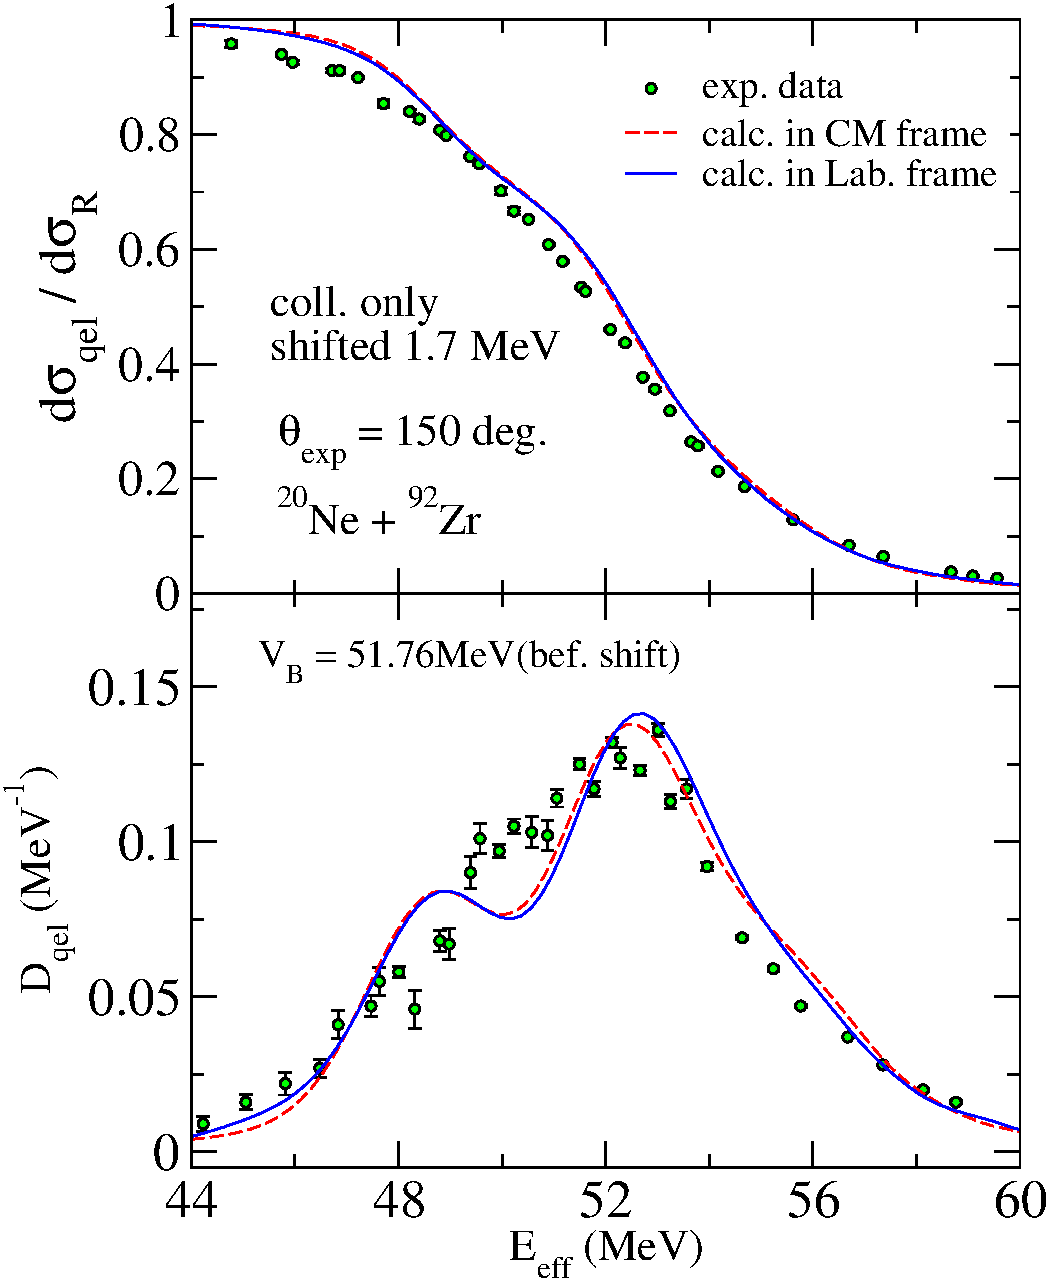
\includegraphics[clip,keepaspectratio,width=100mm]{figure/appendix/qel_20Ne_92Zr_angle_comp.pdf}
%     \caption{Quasi-elastic scattering cross section and barrier distribution for
%     $^{20}$Ne + $^{92}$Zr system. The dots represents the experimental
%     data\cite{evers} at the scattering angle $\theta_{\rm CM}=150^{\circ}$.
%     The red dashed lines are calculated results
%     represented in the CM angles and the
%     blue lines are those in the laboratory frame. 
%     The calculations includes only the
%     collective excitations of the colliding nuclei.  }
%     \label{figB1}
% \end{figure}
% One can see that, the calculations with $\theta_{\rm CM} = 150^\circ$ and
% $\theta_{\rm lab} = 150^\circ$ show almost same result.
% The low-energy tail of the barrier distribution with
% $\theta_{\rm lab}=150^\circ$ reproduces
% that of the data better as it should be.
% If one compares at smaller angles, the difference becomes larger.


\chapter{Role of noncollective excitations in one-dimensional
barrier penetration problem}
In this appendix, we apply the
random matrix model to a
one-dimensional barrier penetration problem
and discuss the role of noncollective excitations\cite{YHR10}.


\section{Random matrix model for one-dimensional coupled-channels equations}
We consider the following coupled-channels equations 
\begin{eqnarray}
  \left\{-\frac{\hbar^2}{2\mu}\frac{d^2}{dx^2} + V_{\rm rel}(x)
  + \epsilon_n - E \right\}\psi_n(x)
  + \sum_m V_{nm}(x)\psi_m(x) = 0.
  \label{cceq}
\end{eqnarray}
Here, $\mu$ is the reduced mass, $V_{\rm rel}(x)$ is a potential for the
relative motion, and $\epsilon_n$ is an excitation energy
for the $n$th channel.

We impose the following boundary condition
\begin{align}
  \psi_n(x) &\rightarrow \delta_{n,0}\,e^{-ik_0x} + r_n \,e^{ik_nx}\ \ \  
              {\rm for}\ \ \ x\rightarrow +\infty \label{bc1}\\
            &\rightarrow t_n \,e^{-ik_nx}\ \ \ {\rm for}\ \ \ 
             x\rightarrow -\infty, \label{bc2}
\end{align} 
where $\displaystyle k_n=\sqrt{{2\mu (E-\epsilon_n)}/{\hbar^2}}$ is 
the wave number for the $n$th channel, and 0 represents the entrance channel.
We have assumed that 
the projectile is incident from the right hand side of the 
potential barrier. 
With the transmission coefficients $t_n$, 
the penetration probability for the inclusive process is calculated as 
\begin{equation}
P(E) = \sum_n P_n(E) = \sum_n\frac{k_n}{k_0} |t_n|^2. 
\end{equation}
The barrier distribution is obtained by taking the energy derivative of 
$P(E)$, that is, $dP(E)/dE$ \cite{HTB97}. 

We solve the coupled-channels equations Eq. (\ref{cceq}) using the constant
coupling approximation by including both collective and noncollective
excitations. For the collective excitation,
we assume the vibrational coupling, whose matrix element
is given by
\begin{eqnarray}
  (V_{nm}) = F
        \left(
          \begin{array}{rr}
            0  &  1         \\
            1  &  0 
          \end{array}
        \right),
        \label{Vcp_vib}
\end{eqnarray}
where $F$ is a constant.

For the noncollective excitations,
we consider an ensemble of coupling matrix elements 
based on the random matrix theory 
\cite{akw1,akw2,akw3}. 
We assume that the matrix elements are uncorrelated random
numbers obeying a Gaussian distribution with zero mean. 
That is, 
we require that the first and the second moments of the
coupling matrix elements satisfy the following equations
\cite{KPW76}
%
\begin{align}
  &\overline{V_{nm}(x)} = 0 \label{1stmom} \\
  &\overline{V_{rs}V_{nm}} = (\delta_{r,n}\delta_{s,m} +
                                    \delta_{r,m}\delta_{s,n})
                                   g_{nm}
   \label{2ndmom} \\
&  g_{nm}  = \frac{w_0}{\sqrt{\rho(\epsilon_n)\rho(\epsilon_m)}}
                 e^{-\frac{(\epsilon_n - \epsilon_m)^2}{2\Delta^2}},
    \label{fmfac2}
\end{align}
where the overline denotes an ensemble average 
and $\rho(\epsilon)$ is the nuclear level density. 
Here, we have assumed the coordinate independent matrix elements 
according to the constant coupling approximation. 

For the noncollective excitations, we generate
the coupling matrix elements according to these equations many times.  
For each coupling matrix, 
we do not vary 
the matrix elements for the 
collective excitations, 
which 
are uniquely determined once 
the coupling is specified.
For each coupling matrix, we solve the coupled-channels 
equations and calculate the penetrability and the reflection 
probability. 
The physical results are then obtained by taking an average of 
these quantities. 



\section{Results}
In solving the coupled-channels equations,
we assume that there is a collective vibrational state at 
1 MeV, whose coupling to the ground state is 
given by Eq. (\ref{Vcp_vib}) with 
$F = 2$ MeV. 
For the noncollective states, 
we consider 
a level density given by 
$\rho(\epsilon) = \rho_0\ e^{2\sqrt{a\epsilon}}$ with  
$\rho_0 = 0.039\ {\rm MeV^{-1}}$ and $a = 29/8\ {\rm MeV^{-1}}$, 
starting from 2 MeV. 
The value of $\rho_0$ was determined so that the number of 
noncollective levels 
is 200 up to 5 MeV. 
For the 
parameters for the couplings in Eq. (\ref{fmfac2}), we 
follow Ref. \cite{KPW76} to use $\Delta$=7 MeV. 
We arbitrarily choose the coupling strength to be 
$w_0 = 0.005$ MeV. 
The energy spectrum for this model is shown in Fig.\ref{fig:spectrum}.
For the potential for the relative motion, $V_{\rm rel}(x)$, 
we use a Gaussian function
%
\begin{equation}
  V_{\rm rel}(x) = V_{\rm B} e^{-\frac{x^2}{2s_0^2}}, 
\label{relgaus}
\end{equation}
%
with $V_{\rm B}$ = 100 MeV and $s_0$ = 3 fm \cite{DLW83}. 
The reduced mass $\mu$ is taken to be 29$m_N$, $m_N$ being the 
nucleon mass. 

\begin{figure}[hb]
  \begin{center}
    \includegraphics[clip,keepaspectratio,width=80mm]{figure/appendix/fig1.eps}
    \caption{The energy spectrum for the model 
             calculation which we employ. 
             There is a collective vibrational state at 1 MeV, while 
             noncollective states exist from 2 MeV with an exponentially 
             increasing level density. }  
    \label{fig:spectrum}
  \end{center}
\end{figure}

Figure \ref{fig:penet} shows the penetrabilities thus obtained.
The corresponding barrier distributions 
are shown in 
Fig. \ref{fig:bardist}. 
The dotted and the dashed lines show the results  
without the channel couplings and those only with the collective 
excitation, respectively. 
The solid line shows the results with both the noncollective excitations and 
the collective excitation. 
We include the noncollective states up to $\epsilon_{\rm max}=$23 MeV with 
energy spacing of $\Delta \epsilon$=0.02 MeV. 
This result is obtained by 
generating 
the coupling matrix elements 30 times to take an ensemble average. 

The collective excitation leads to a double peaked structure 
of barrier distribution. 
One can see that the noncollective excitations 
suppress the penetrability at energies above the barrier, and 
at the same time smear the higher energy peak in the 
barrier distribution, although the main structure of the barrier 
distribution is still determined by the collective excitation. 
The noncollective excitations also lower the barrier and thus 
increase the penetrability at energies below the barrier, due to 
the potential renormalization discussed in chapter 3. 

\begin{figure}[t]
  \begin{center}
    \begin{minipage}[t]{77mm}
      \includegraphics[clip,keepaspectratio,width=77mm]{figure/appendix/fig2.eps}
      \caption{The potential penetrability obtained with several methods. 
The dotted line is obtained without channel coupling, while 
the dashed line takes into account only the collective vibrational 
excitation. The solid line shows the result with 
both the collective and the noncollective excitations.}
      \label{fig:penet}
    \end{minipage}
    \hspace{0.5cm}
    \begin{minipage}[t]{79mm}
       \includegraphics[clip,keepaspectratio,width=79mm]{figure/appendix/fig3.eps}
       \caption{The barrier distribution defined by the first derivative 
of the penetrability. The meaning of each line is the 
same as in Fig.\ref{fig:penet}.}
       \label{fig:bardist}
    \end{minipage}
  \end{center}
\end{figure}

The $Q$-value distribution for the reflected flux is shown in 
Fig. \ref{fig:qdist} at four incident energies indicated in the figure. 
For a presentation purpose, we fold the discrete 
distribution with a Lorentz function, 
\begin{eqnarray}
  f(\epsilon) = \frac{1}{\pi}\frac{\eta}{\epsilon^2 + \eta^2},
\end{eqnarray}
with the width of $\eta=$0.2 MeV. 
%
In the figure, 
the peaks at $E^{*}=0\ {\rm MeV}$ and $E^{*}=1\ {\rm MeV}$ correspond to the 
elastic channel and the collective excitation channel, respectively.
One can see that at energies well below the barrier 
the elastic and the collective peaks dominate in the distribution. 
As the energy increases, the 
single-particle excitations become more and more important. 
This behaviour is consistent with the experimental $Q$-value 
distribution observed for $^{16}$O+$^{208}$Pb \cite{evers,lin} 
and $^{16}$O+$^{184}$W \cite{lin} reactions.  
At energies above the barrier, the noncollective contribution is even larger than 
the contribution of the elastic and the collective peaks. 

\begin{figure}[t]
    \center
    \includegraphics[clip,keepaspectratio,width=80mm]{figure/appendix/fig4.eps}
    \caption{The $Q$-value distribution for the reflected flux at four energies 
as indicated in the figure. It is obtained by smearing the discrete 
distribution with a Lorentzian function with the width of 0.2 MeV. 
The peaks at $E^{*}$=0 MeV and
      1 MeV correspond to the elastic and the 
collective excitation channels, respectively.}
    \label{fig:qdist}
\end{figure}






\chapter{Calculation of gaussian orthogonal ensemble(GOE)}
In this appendix, we present a calculation method for
the coupling matrix elements according 
to the random matrix theory\cite{BDK95}.
The second moment of the coupling matrix elements is
assumed to be given by 
Eq. (\ref{goe_2}) as
\begin{eqnarray}
\overline{V_{nn^\prime}^{II^\prime}(r)V_{n^{\prime\prime}n^{\prime\prime\prime}}^{I^{\prime\prime}I^{\prime\prime\prime}}(r^\prime)}
&=& \left\{\delta_{nn^{\prime\prime}}\delta_{n^{\prime}n^{\prime\prime\prime}} 
          \delta_{II^{\prime\prime}}\delta_{I^{\prime}I^{\prime\prime\prime}}
   + \delta_{nn^{\prime\prime\prime}}\delta_{n^{\prime}{n^{\prime\prime}}}
                      \delta_{II^{\prime\prime\prime}}\delta_{I^{\prime}{I^{\prime\prime}}}
   \right\}
   \sqrt{(2I+1)(2I^\prime+1)}   \nonumber\\
& & \times \sum_{\lambda}
   \left(
     \begin{array}{ccc}
       I & \lambda & I^{\prime} \\
       0 & 0 & 0
     \end{array}
   \right)^{2}
\alpha_{\lambda}(n,n^\prime;I,I^\prime;r, r^\prime)
\label{AppC1}
\end{eqnarray}
with the form factor 
\begin{eqnarray}
\alpha_{\lambda}(n,n^\prime;I,I^\prime;r, r^\prime) =
\frac{w_\lambda}{\sqrt{\rho(n,I)\rho(n^\prime,I^\prime)}}
e^{-\frac{(\epsilon_n-\epsilon_n^\prime)^2}{2\Delta^2}}
e^{-\frac{(r-r^{\prime})^2}{2\sigma^2}}
h(r)h(r^{\prime}).
\label{AppC2}
\end{eqnarray}
In order to construct $V_{nn^\prime}^{II^\prime}(r)$ which satisfies Eq.
(\ref{AppC1}), we define the following function
\begin{eqnarray}
g_{nn^{\prime}}^{II^{\prime}}(r, r^{\prime})
=
\sqrt{
   \sum_{\lambda}
   \left(
     \begin{array}{ccc}
       I & \lambda & I^{\prime} \\
       0 & 0 & 0
     \end{array}
   \right)^2
   w_\lambda
\sqrt{
\frac{(2I+1)(2I^{\prime}+1)}{\rho(n,I)\rho(n^{\prime},I^{\prime})}
}
}
e^{-\frac{(\epsilon_{n}-\epsilon_{n^{\prime}})^2}{4\Delta^2}}
h(r)
\left(\frac{2}{\pi\sigma^2}\right)^{1/4}
e^{-\frac{(r-r^{\prime})^2}{\sigma^2}},
\end{eqnarray}
which corresponds to the "square root" of the form factor $\alpha_{\lambda}$.
Using this function, the coupling matrix element is calculated as
\begin{align}
V_{nn^\prime}^{II^\prime}(r) 
= \int dr^{\prime} g_{nn^{\prime}}^{II^{\prime}}(r, r^{\prime})
  w_{nn^{\prime}}^{II^\prime}(r^\prime),
  \label{AppC4}
\end{align}
where $w_{nn^\prime}(r)$ is a gaussian random number which satisfies
\begin{align}
\overline{w_{n_1n_2}(r) w_{n_3n_4}(r^\prime)}
= \left(\delta_{n_1n_3}\delta_{n_2n_4} + \delta_{n_1n_4}\delta_{n_2n_3}\right)
  \delta(r - r^\prime).
\end{align}
The gaussian random numbers can be generated from uniform random numbers
distributed in the interval $(0,1]$ by, for instance, the Box-Muller method.
That is, from the independent 
random numbers $x_1$ and $x_2$ uniformly distributed 
in the interval $(0,1]$,
the independent random numbers
$y_1$ and $y_2$ with a gaussian distribution 
are generated by the following equations\cite{numerical}
\begin{align}
y_1 &= \sqrt{-2{\rm ln}\,x_1}{\rm cos}(2\pi x_2) \\
y_2 &= \sqrt{-2{\rm ln}\,x_1}{\rm sin}(2\pi x_2).
\end{align}
It is a straightforward task to verify that the
coupling matrix element defined by
Eq. (\ref{AppC4}) satisfies Eq. (\ref{AppC1}).




\chapter{Interplay of collective and noncollective excitations}
In this appendix, we discuss the interplay of collective and noncollective
excitations by using a schematic model.
Depending on the type of the collective excitations which dominate the barrier
structure, the effect of the noncollective excitations
on the barrier distribution appears
differently.
In order to investigate this difference, 
we consider three cases where the
collective excitations are vibration, 
rotation associated with a prolate deformation,
and rotation associated with an oblate deformation.
We also use the perturbation theory to 
give an interpretation for the
effect of the noncollective excitations on the barrier distribution.
The purpose of this appendix is to gain an insight of
the smearing effect of the noncollective excitations
observed in the $^{20}$Ne + $^{92}$Zr system, where the 
rotational excitations 
with prolate deformation dominate the barrier structure.
To this end, we use a constant
coupling approximation and work in the eigenchannel
representation, which makes an interpretation of the
noncollective effects transparent.
In this representation, 
we shall see whether the shrinkage of the peaks in
the barrier distribution,
which leads to the smearing of the barrier structure,
occurs due to the noncollective excitations.
Although we consider the collision of $^{20}$Ne + $^{92}$Zr system, 
the collective excitation channels are artificially
modified for $^{92}$Zr nucleus,
while the realistic noncollective states of
$^{92}$Zr are included in the same
way as in the calculations shown in chapter 6.
$^{20}$Ne is assumed to be inert.

We first consider the rotational excitations.
We set the excited states with the
excitation energy $\epsilon_2 = 0.4$ MeV and the deformation
parameter $\beta_2 = \pm0.25$.
The potential parameters are the same as in the previous calculations for
$^{20}$Ne + $^{92}$Zr system.
We show the fusion barrier
distributions for the case of prolate deformation
($\beta_2 > 0$) in Figs. \ref{fig7.23}(a) and \ref{fig7.24}(a)
and oblate deformation ($\beta_2 < 0$)
in Figs. \ref{fig7.25}(a) and \ref{fig7.26}(a).
The red lines include only the collective excitations and the blue lines
include the noncollective excitations in addition to the collective
excitations.
Fig. \ref{fig7.23} shows the results when the rotational states
are truncated at the $2^+$ state and
Fig. \ref{fig7.24} takes into account up to the $4^+$ state.
As mentioned in chapter 3, 
we can introduce the eigenchannel representation when
the constant coupling approximation is employed.
The magenta and the cyan spectra represent
eigenbarriers respectively for
the red and the blue calculations.
In Fig.\ref{fig7.23}(a), 
the difference of the height of the two
eigenbarriers is $\Delta\lambda = 5.14$ MeV as indicated in the figure. If we
take into account the noncollective excitations,
the difference decreases and becomes
$\Delta\lambda$ = 4.71 MeV.
This is also the case if one include the 
rotational $4^+$ states in addition, that
is, the distance between the lowest two eigenbarriers decreases.
\begin{figure}[h]
  \center
  \begin{minipage}[t]{78mm}
    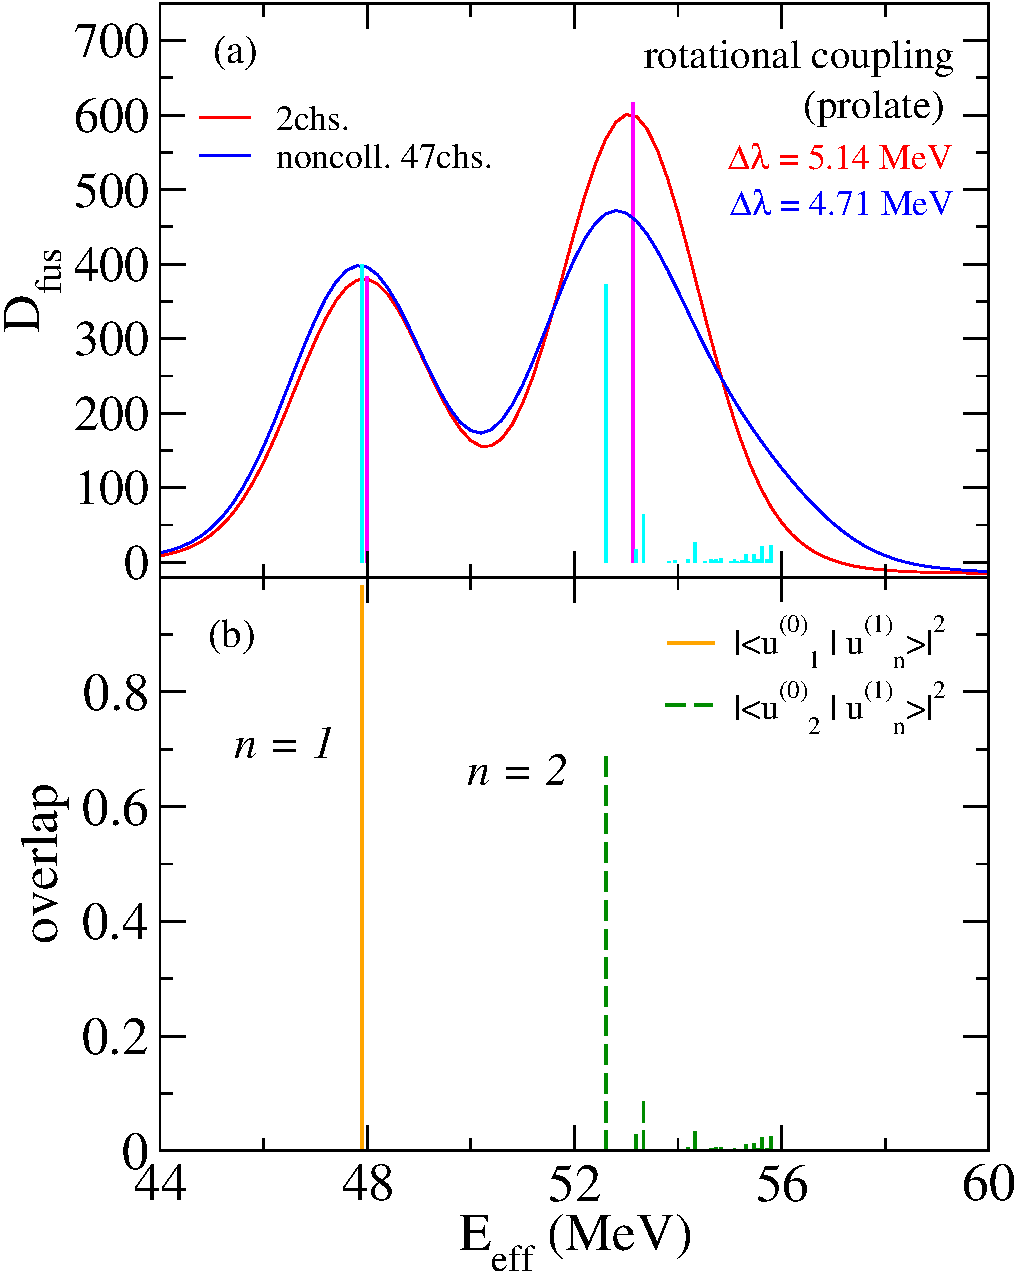
\includegraphics[clip,keepaspectratio,width=78mm]{figure/appendix/fus_prolate_2ch.pdf}
    \caption{The upper panel: Fusion barrier distributions for
    a rotational coupling associated
    with a prolate deformation.
    The rotational states are included up to the 2$^+$ state.
    The red line includes only the collective excitations
    while the blue one includes also the
    noncollective excitations. The pink and the cyan spectra represent the
    position of the eigenbarriers corresponding 
    to the red and the blue lines, respectively.
    The lower panel: The overlap of the perturbed and the unperturbed
    eigenvectors for a prolate rotational coupling.
    The orange and the purple lines represent
    the overlap with the eigenvector belonging
    to the lowest and the second lowest 
    unperturbed eigenvalues, respectively.}
    \label{fig7.23}
  \end{minipage}
  \hspace{0.5cm}
  \begin{minipage}[t]{78mm}
    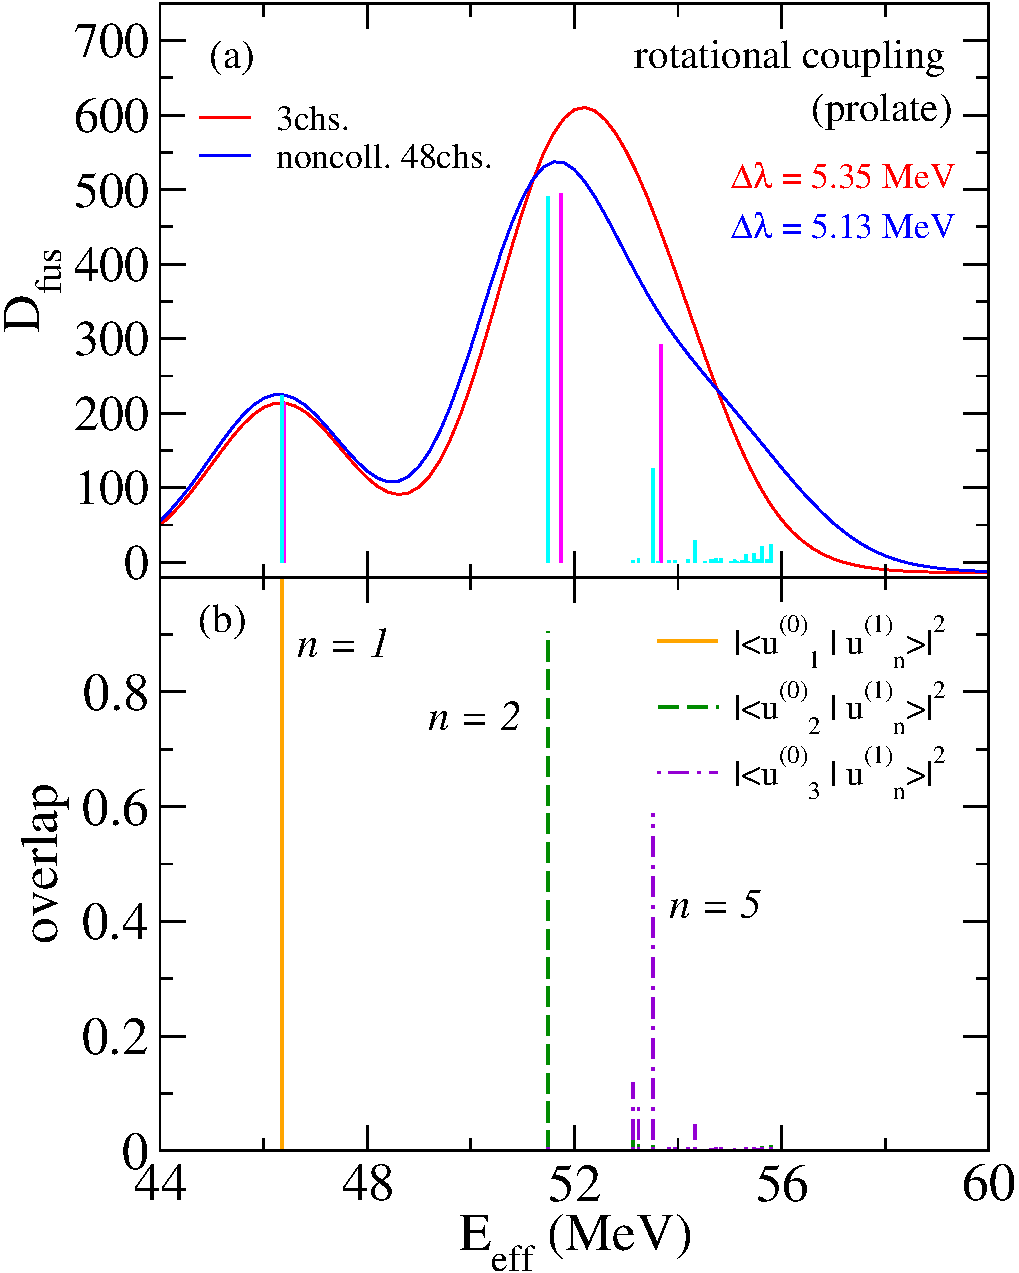
\includegraphics[clip,keepaspectratio,width=78mm]{figure/appendix/fus_prolate_3ch.pdf}
    \caption{Same as Fig. \ref{fig7.23}, but with the $4^{+}$ state
    in the rotational coupling. The green lines in the lower panel represent the 
    overlap with the eigenvector belonging to the third lowest unperturbed
    eigenvalues.}
    \label{fig7.24}
  \end{minipage}
\end{figure}

We show the overlap spectra for
prolate deformation case in Figs. \ref{fig7.23}(b) and \ref{fig7.24}(b)
and oblate deformation cases in Figs. \ref{fig7.25}(b) and \ref{fig7.26}(b).
The orange, the green, and the purple (only in Figs. \ref{fig7.24}(b) and
\ref{fig7.26}(b)) lines are the
overlap between the unperturbed
(in the absence of the noncollective excitations)
and the perturbed (in the presence of the noncollective excitations)
eigenvectors.
The horizontal axis represents the height of the eigenbarriers in the presence of the
noncollective excitations.
We can see that the unperturbed eigenvector 
for the lowest eigenbarrier has largest overlap with
the perturbed eigenvector for $n=1$, that is, the lowest eigenbarrier.
Similarly, the unperturbed eigenvector for the second lowest eigenbarrier has
the largest overlap with the perturbed eigenvector for $n=2$.
\begin{figure}[t]
  \center
  \begin{minipage}[t]{78mm}
    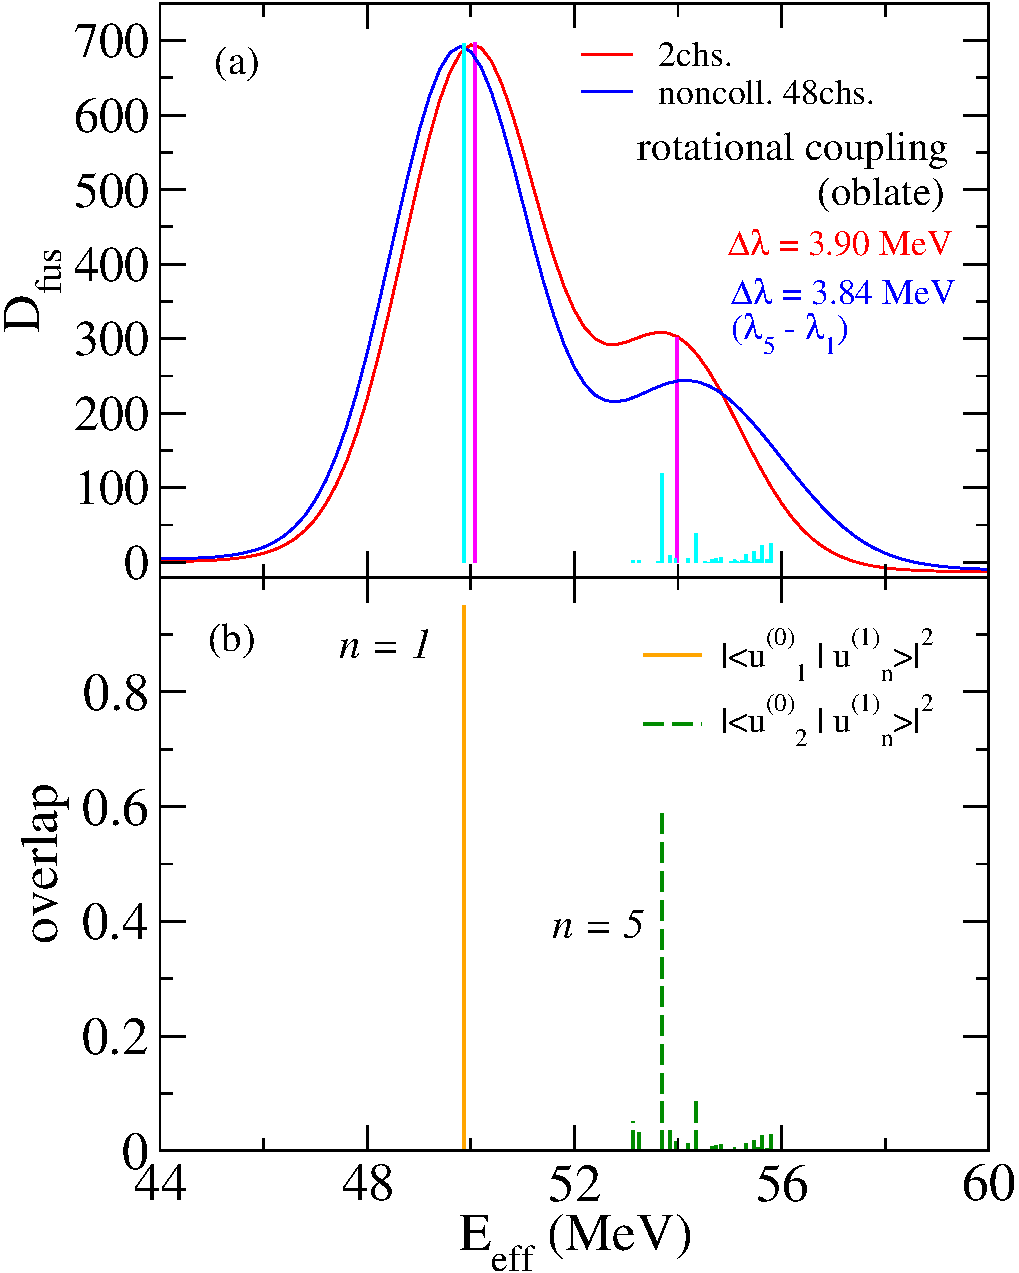
\includegraphics[clip,keepaspectratio,width=78mm]{figure/appendix/fus_oblate_2ch.pdf}
    \caption{Same as Fig.\ref{fig7.23}, but for an oblate deformation.}
    \label{fig7.25}
  \end{minipage}
  \hspace{0.5cm}
  \begin{minipage}[t]{78mm}
    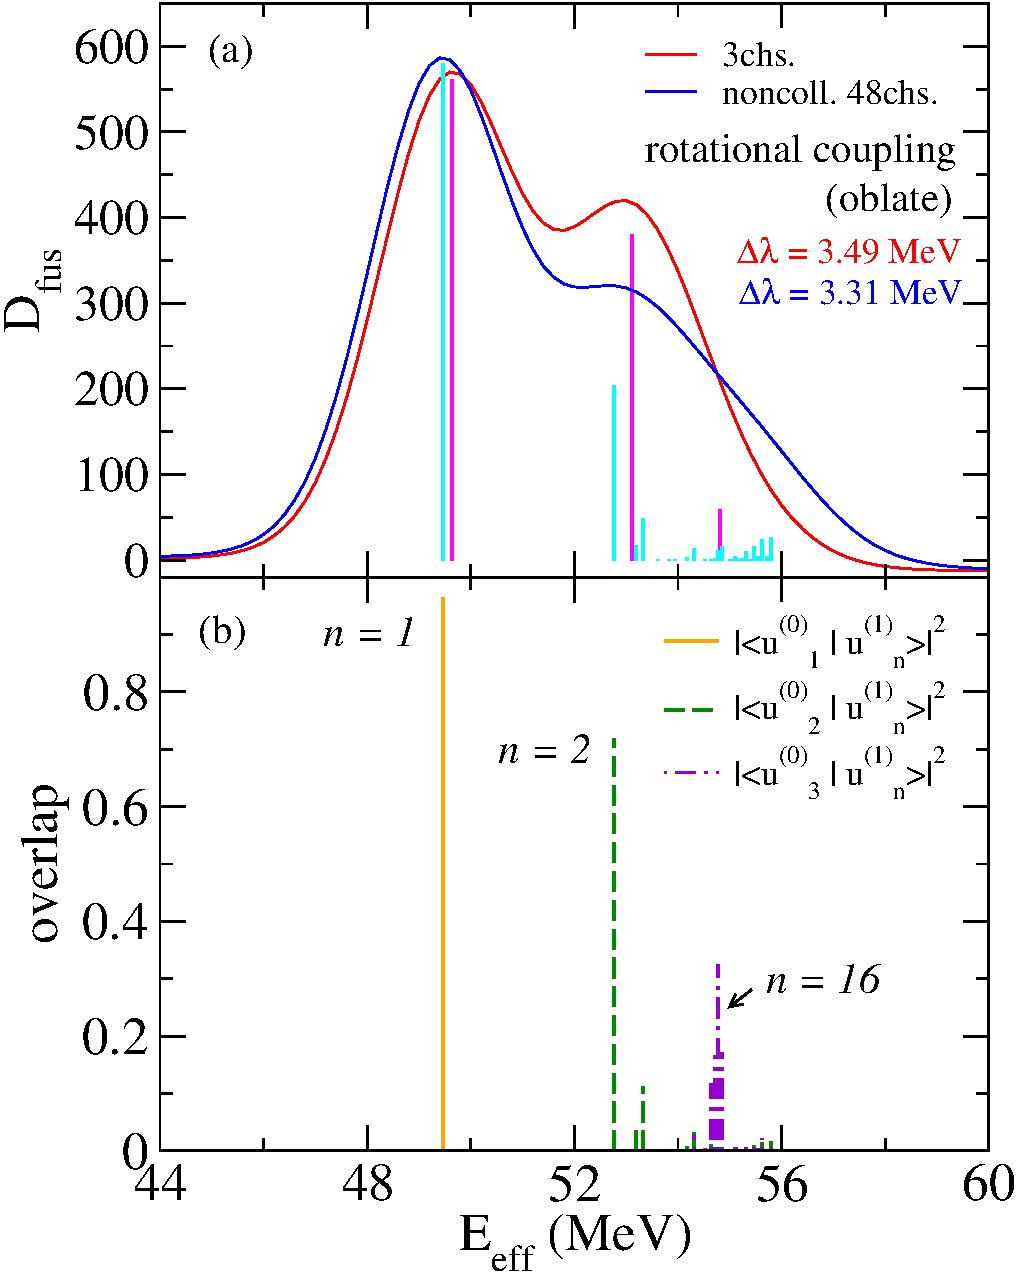
\includegraphics[clip,keepaspectratio,width=78mm]{figure/appendix/fus_oblate_3ch.pdf}
    \caption{Same as Fig.\ref{fig7.24}, but with an oblate deformation.}
    \label{fig7.26}
  \end{minipage}
\end{figure}

For an oblate deformation with the 0$^+$ and 2$^+$ states,
we can see that by including the noncollective excitations,
the distance between the eigenbarriers becomes slightly smaller.
On the other hand, including the rotational states up to the 4$^+$ state,
the higher peak is fragmented and
the distance of the peaks in the barrier
distribution appears to be
broadened by including the noncollective excitations, in contrast
to the prolate case.
A similar behavior can be observed for the vibrational coupling case.
In Figs. \ref{fig7.27} and \ref{fig7.28}, we show the same calculation for the
vibrational coupling case.
We assume that the vibrational 2$^+$ state is located at $\epsilon_2
= 1.0$ MeV in $^{92}$Zr nucleus with
a deformation parameter of $\beta_2 = 0.25$.
Fig. \ref{fig7.27} includes only one phonon state
for the vibrational coupling and
Fig. \ref{fig7.28} includes the two phonon state
in addition to the one phonon state.
The meaning of each line is the same as the rotational case.
Although the distance between the eigenbarriers becomes smaller
(4.18 MeV to 3.91 MeV) by including the noncollective excitations,
the peak distance of the barrier distribution appears to be broadened.
The highest eigenbarrier gains a relatively large weight both for the
rotational coupling with oblate 
deformation and vibrational coupling cases, and this
makes the peak distance broad.
However, for the rotational coupling with a prolate deformation, the highest
eigenbarrier does not broaden the main peaks.
This is because in the prolate deformation case, the higher eigenbarrier has a
larger weight in the unperturbed calculation, and the highest eigenbarrier which
appears in the perturbed calculation only smear the higher peak of the barrier
distribution and does not broaden the peak distance.
\begin{figure}[t]
  \center
  \begin{minipage}[t]{78mm}
    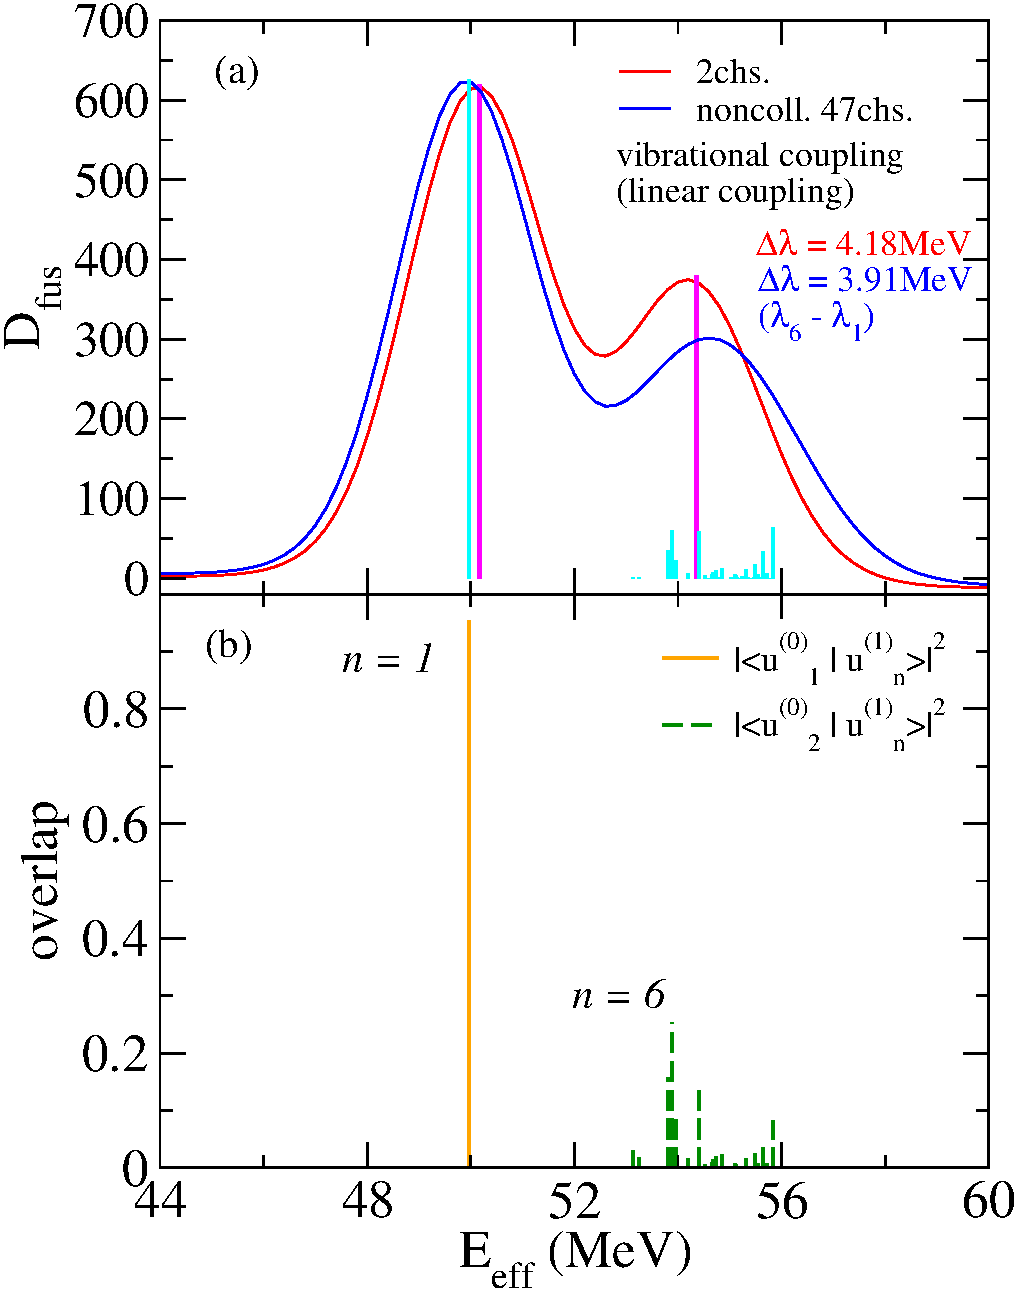
\includegraphics[clip,keepaspectratio,width=78mm]{figure/appendix/fus_vibration_linear_2ch.pdf}
    \caption{Same as Fig. \ref{fig7.23}, but with a vibrational coupling.}
    \label{fig7.27}
  \end{minipage}
  \hspace{0.5cm}
  \begin{minipage}[t]{78mm}
    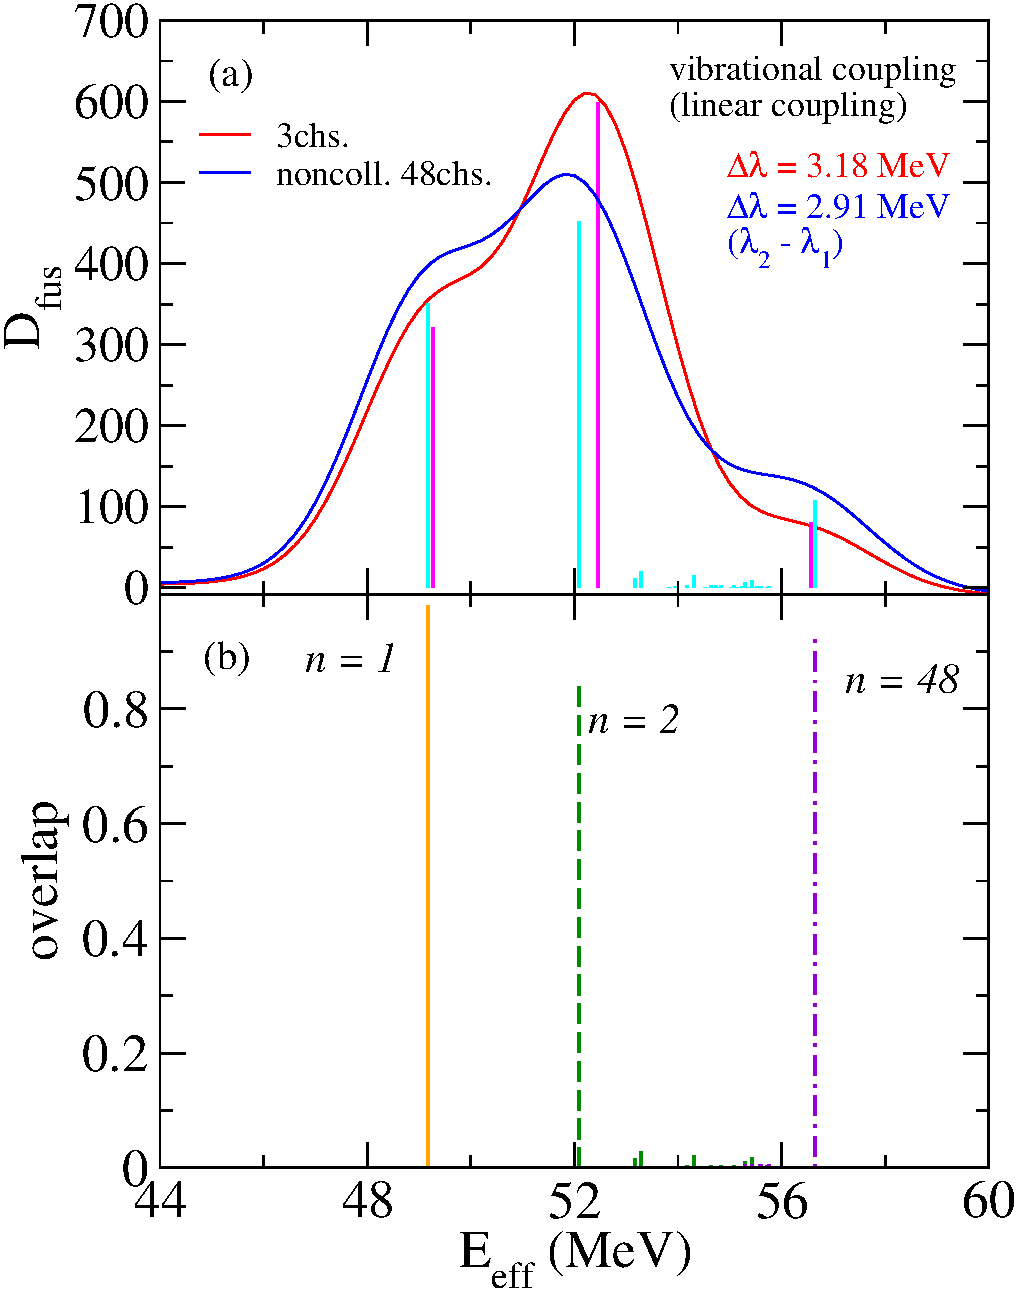
\includegraphics[clip,keepaspectratio,width=78mm]{figure/appendix/fus_vibration_linear_3ch.pdf}
    \caption{Same as Fig. \ref{fig7.24}, but with a vibrational coupling.}
    \label{fig7.28}
  \end{minipage}
\end{figure}

We can give some explanation to the shrinkage of the peak distance for the
rotational coupling with a prolate deformation according
to the perturbation theory.
The coupling matrix in the present calculation has the following form
\begin{eqnarray}
V = (V_{\rm coll} + \bvec{\epsilon}) + V_{\rm RMT}
\end{eqnarray}
with
\begin{eqnarray}
V_{\rm coll} + \bvec{\epsilon} =
\left(
\begin{array}{ccccc}
0 & f & 0 & 0 &  \cdots\\
f & g & 0 & 0 &  \cdots\\
0 & 0 & \epsilon_3  & 0 & \cdots \\
0 & 0 & 0 & \epsilon_4  & \cdots \\
\vdots & \vdots & \vdots & \vdots  & \ddots
\end{array}
\right)
\end{eqnarray}
and 
\begin{eqnarray}
V_{\rm RMT} =
\left(
\begin{array}{ccccc}
0 & 0 & c_3 & c_4 &  \cdots\\
0 & 0 & 0 & 0 &  \cdots\\
c_3 & 0 & 0 & 0 & \cdots \\
c_4 & 0 & 0 & 0 & \cdots \\
\vdots & \vdots & \vdots & \vdots  & \ddots
\end{array}
\right).
\end{eqnarray}
The first matrix represents the coupling matrix
related to the collective excitation
plus excitation energy (the unperturbed part),
and the second matrix represents the
coupling matrix related to the noncollective
excitations (the perturbed part).
The numbers $f, g, c_3, c_4, \cdots$ represent
the coupling strength ($g$ includes the excitation energy 
of the collective state $\epsilon_2$), and 
$\epsilon_3, \epsilon_4, \cdots$ represents the excitation energies of the
noncollective states.
One can diagonalize the unperturbed coupling matrix by some unitary matrix $U$
as
\begin{eqnarray}
U\left\{V_{\rm coll} + \bvec{\epsilon}\right\}U^{\dagger} =
\left(
\begin{array}{ccccc}
\lambda_1^{(0)} & 0 & 0 &   \cdots\\
0 & \lambda_2^{(0)} & 0 &   \cdots\\
0 & 0 & \lambda_3^{(0)} &  \cdots \\
\vdots & \vdots & \vdots  & \ddots
\end{array}
\right),
\end{eqnarray}
and the unitary matrix $U$ has the form
\begin{eqnarray}
U =
\left(
u_1^{(0)}, u_2^{(0)}, u_3^{(0)}, \cdots \right) 
=
\left(
\begin{array}{ccccc}
u_{11}^{(0)} & u_{12}^{(0)} & 0 & 0&  \cdots\\
u_{21}^{(0)} & u_{22}^{(0)} & 0 & 0&  \cdots\\
0 & 0 & 1 & 0& \cdots \\
0 & 0 & 0 &1 &  \cdots \\
\vdots & \vdots &\vdots & \vdots  & \ddots
\end{array}
\right).
\end{eqnarray}
Note that $\lambda_m^{(0)} = \epsilon_m$ for $m \ge 3$.
Here, we make an assumption that $\lambda_2^{(0)} \le \lambda_m^{(0)}(m \ge 3)$.
The first order perturbation theory gives zero and the second order perturbation
gives
\begin{eqnarray}
\lambda_n^{\prime} = \lambda_n^{(0)}
+ \sum_{m\ne n}
\frac{\left|\langle u_n^{(0)} | V_{\rm RMT} | u_m^{(0)} \rangle \right|^2}
{\lambda_n^{(0)} - \lambda_m^{(0)}}.
\end{eqnarray}
We consider the difference of $\lambda_1^{\prime}$ and $\lambda_2^{\prime}$.
It is given by
\begin{eqnarray}
\lambda_2^{\prime} - \lambda_1^{\prime} =
\lambda_2^{(0)} - \lambda_1^{(0)}
+\sum_{m \ge 3}
\frac{\lambda_1^{(0)} - \lambda_m^{(0)}
+\left(2\lambda_m^{(0)} - \lambda_1^{(0)} - \lambda_2^{(0)} \right){u_{11}^{(0)}}^2}
{\left(\lambda_1^{(0)} - \lambda_m^{(0)}\right)\left(\lambda_2^{(0)} -
\lambda_m^{(0)}\right)} c_m^2
\end{eqnarray}
From this equation, we can say that
if
\begin{eqnarray}
{u_{11}^{(0)}}^2 \le \frac{\lambda_m^{(0)} -
\lambda_1^{(0)}}{2\lambda_m^{(0)} - \lambda_1^{(0)} - \lambda_2^{(0)}}
\label{condition}
\end{eqnarray}
is satisfied for at least all $m \ge 3$, then
\begin{eqnarray}
\lambda_2^{\prime} - \lambda_1^{\prime} \le \lambda_2^{(0)} - \lambda_1^{(0)},
\end{eqnarray}
that is, the distance of the eigenbarrier becomes smaller.
Notice that the left hand side of the condition (\ref{condition}) is the weight
factor for the lowest eigenbarrier.
In the case of a rotational coupling with a prolate deformation considered above,
the assumption with respect to the ordering of $\lambda_n^{(0)}$ is satisfied.
In addition, from
\begin{eqnarray}
\frac{\lambda_m^{(0)} -
\lambda_1^{(0)}}{2\lambda_m^{(0)} - \lambda_1^{(0)} - \lambda_2^{(0)}}
\ge
\frac{\lambda_m^{(0)} -
\lambda_1^{(0)}}{2\left(\lambda_m^{(0)} - \lambda_1^{(0)}\right)} = \frac{1}{2},
\end{eqnarray}
and the fact that the lower eigenbarrier has a smaller
weight factor than that of the 
higher one in the case of prolate deformation,
the condition (\ref{condition}) is satisfied.
Thus, the perturbation theory predicts the shrinkage of the distance between
the eigenbarriers, and as we have seen above, this is the case.
For the case of a rotational coupling with 
an oblate deformation and a vibrational
coupling, the lower eigenbarrier has a larger weight factor and the condition
(\ref{condition}) is not necessarily satisfied, even if the assumption with
respect to the ordering of the eigenbarriers is satisfied.
Thus, we cannot draw a definite conclusion in contrast to
the prolate deformation case.

Generally speaking from the discussion in this sections, it is clear
that the shrinkage of the peak distance due to the noncollective excitations,
which leads to the smearing of the peak structure, 
tends to be occurred for the
reaction with the rotational coupling associated with prolate deformation.

\end{document}

